 \documentclass{tlp}
  \usepackage{aopmath}
  \usepackage{url}
  \usepackage{epsfig}
  \usepackage{psfig}

  \DeclareGraphicsRule{.gif}{eps}{}{}
  
  \begin{document}
   \bibliographystyle{acmtrans}


\title{A Reasoner for the Web}
\author[Berners-Lee et. al.]{Tim Berners-Lee \and Dan Connolly \and James Hendler \and Vladimir Kolovski \and Yoseph Scharf}
  \maketitle
\label{firstpage}
  

    \begin{abstract}
  


\par Cwm (pronounced coom) is a general-purpose data processor for
the semantic web, somewhat like sed, awk, etc. for text files or
XSLT for XML. It is a forward chaining reasoner which can be used
for querying, checking, transforming and filtering information. Its
core language is RDF, extended to include rules, and it uses
RDF/XML or RDF/N3 serializations as required. The logic, and the
functions To be used effectively as a Semantic Web reasoner, Cwm
has a host of features that allow it to operate as an agent on the
Semantic Web . In this paper, we discuss those features and show
why we consider cwm a reasoner for the Semantic Web.
\end{abstract}
  


\section{Introduction: Motivation and Goals}
  

\par The popularity of the Semantic Web is ever-increasing, one of
the main reasons being the improving tool support for its
foundational languages (OWL and RDF). This tool support usually
comes in the form of ontology editors and reasoners for
OWL\footnote{because of its clear and concise semantics,
 OWL-DL can boast a large number of reasoners.}.
However, for the general
purpose manipulation of data, a rule-based engine makes intuitive
things which are unintuitive, difficult or sometimes impossible
using Description Logics. The requirements for such a rule engine
were twofold: to be a general tool to allow semantic-web based
systems to be built, so as to provide feedback on the overall
architecture, and provide an on-ramp for newcomers; and to provide
a platform on which to build more sophisticated applications to
research future directions for semantic web design.

\par In the context of the Semantic Web, RDF is the lingua franca for
representing machine-processable documents. RDF uses URIs as
symbols. The {\it Web} in Semantic {\it Web} comes from the fact
that from your document you can link to just about any web resource
you like. However, the Web contains many sources of information,
with different characteristics and relationships to any given
reader. Whereas a closed system may be built based on a single
knowledge base of believed facts, an open web-based system exists
in an unbounded sea of interconnected information resources. This
requires that an agent be aware of the provenance of information,
and responsible for its disposition. A tool in this type of
environment should have the ability to determine what document or
message said what and match graphs against variable graphs.

\par The goal of the Semantic Web is the beneficial reuse of data in
unplanned ways. (@@this is discussed in the N3 section)

\par We introduce a tool called Cwm [footnote: originally from Closed
World Machine, now a misnomer, as cwm explicitly deals with open
world.] motivated by the above requirements. Cwm is a
general-purpose data processor for the semantic web, analogous like
sed, awk, etc. for text files or XSLT for XML. It is a forward
chaining reasoner which can be used for querying, checking,
transforming and filtering information. Since RDF itself is not
sufficient to express rules, Cwm is based on an extension of RDF
called Notation3 (N3) which has support for quoting (making
statements about statements), variables and rules.

\par Being based on a more expressive logic language added a host of
features to Cwm not available to other RDF processing tools:
possibility of filtering RDF graphs after merging them, for
example. Since N3 is expressive enough so that positive
datalog-like rules can be expressed in it, cwm is able to reason
using a first order logic but without classical negation. Combining
this reasoning functionality with its ability to retrieve documents
form the web as needed, the system can be considered a reasoner for
the web. It has grown from a proof of concept application to a
popular rule engine, used in major research projects. The goal of
this paper is to explain the functionality and distinguishing
features of this tool in more detail.

\par The second goal cwm, as a platform for research, was in a way to
serve as a experimental ground for more expressive Semantic Web
applications (which cover some of the upper layers of the Semantic
Web layer cake). To this end, we have added {\it proof}
generation/checking support to the system, and also a crypto module
which empowers Cwm users with the tools to build {\it trust}
systems on the Semantic Web.

\par In the next section there will be a brief introduction to N3,
mainly describing how it extends RDF. Then, we will briefly explain
the system architecture of cwm. From that point on, we will talk
about the distinguishing features of the tool, such as its builtin
functions, proof generation and proof checking. Cwm has been used
as the rule engine in research projects (Policy Aware Web) and for
automating tasks at the W3C - we will cover that in Applications,
and wrap up with Future Work and Conclusions.




\section{Preliminaries: N3}
  

\par Notation3 (N3) is a language which is a compact and readable
alternative to RDF's XML syntax, but also is extended to allow
greater expressiveness. It has two important subsets, one of which
is RDF 1.0 equivalent, and one of which is RDF extended with rules.
In this section, we will briefly introduce N3 show how it is
different from RDF.

\par N3 syntax is very readable, using the <subject>
<predicate> <object> form. E,g.:

\par {\tt :John :parent :Bob.}

\par The colon form of qname is similar to XML's qname form. In this
paper, for the sake of space, we do not define the namespaces to
which prefxes refer. [@@in a footnote we could] Blank nodes
(bnodes, RDF's form of existential node) are expressed using '[]',
for example: [ :brother :John ] specifies some person who has
brother :John.

\par An N3 rule is stored as a statement whose predicate is
{\tt log:implies}, for example:
\begin{verbatim}
{ ?x parent ?y. ?y sister ?z } log:implies { ?x aunt ?z }.
\end{verbatim}

\par Set of statements surrounded by braces is called an N3 formula.
Formula is a generalization of an RDF-graph, adding variables.

\par N3 rules are at the same time more and less expressive than
Datalog. On one hand, N3 is restricted to binary predicates
(triples), but on the other, existentials (bnodes) are allowed in
the consequents of the rules. Another restriction worth mentioning
is that, since monotonicity is one of the design goals for N3,
there is no negation-as-failure. The only form of negation allowed
in N3 is scoped negation as failure, which will be described in
Section [@@REF].

\par One of the design goals of N3 is that information, such as but
not limited to rules, which requires greater expresive power than
RDF, should be sharable in the same way as RDF can be shared. This
means that one person should be able to express knowledge in N3 for
a certain purpose, and later independently someone else reuse that
knowledge for a different unforeseen purpose. As the context of the
later use is unknown, this prevents us from making implicit closed
assumptions about the total set of knowledge in the system as a
whole. As a result of this, N3 does not make the Closed World
Assumption in general.
\section{Architecture}
  

\par Figure 1 represents a high-level architecture diagram of Cwm. In
the following subsections, we will expand on the most important
sections of the diagram.
\begin{figure}[tb]
\centerline{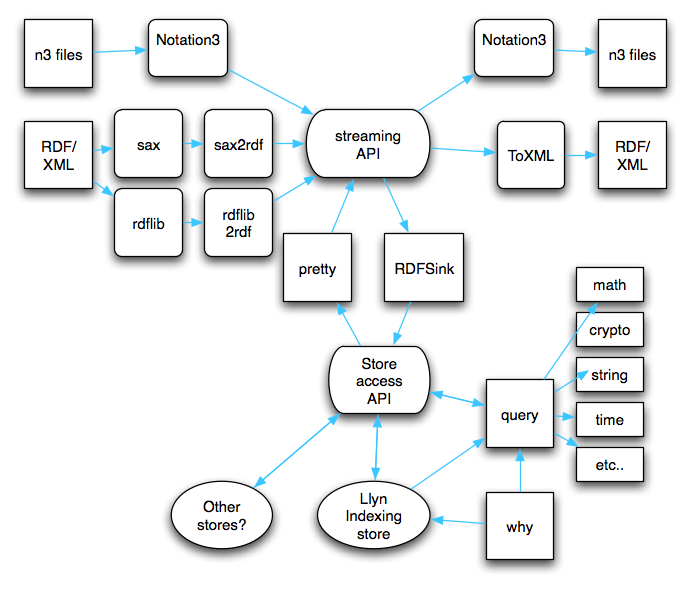
\epsfig{file=CwmArch2.pdf, height=4in}}

\caption{cwm software architecture}\label{cwmarch}

\end{figure}

\subsection{Parsing and Serialization}
  

\par The N3 and RDF languages are grammatically similar, to the
extent that it is possible to translate one into the other in a
streaming mode. The efficiencies evident from this mode of
operation led to a design of an abstract syntax interface which
parsers and serializers supported. This is still in use, but
experience was that as the N3 language became more sophisticated,
the streaming interface became more burdensome to support as an
output format for the serialization module
({\tt pretty.py}).
\subsection{Store}
  

\par The store ({\tt llyn.py}) is a triple store, extended to
cover the full N3 language, and also to record the provenance of
each statement. A statement therefore is stored as the subject,
predicate and object of RDF, plus the '{\em context}' the
identity of the formula in which the statement is, and a record of
the {\em reason} object which stores the reason for the
statement having been added to the store. This is used in proof
processing.

\par The store was originally designed and built with four indices,
so that list was kept of each statement in which a given term
occurred as, respectively, the subject, predicate, object or
context. When there was a need to improve performance, this was
changed so than now 7 indices are used, as almost every combination
of subject , predicate, object pattern with wildcards are indexed.
This is a questionable tradeoff, as many tasks involve the input
and output of data with relatively little processing, so the
indexing overhead may dominate.
\subsection{Inference engine}
  

\par The inference engine is essentially a simple forward chaining
reasoner for N3 rules.

\par The matching engine which runs the rules operates simply by
recursive search, with some optimizations. Firstly, the rule set is
analyzed to determine which rules can possible affect the output of
some other rules. A partial order is found, which for example in
some cases will produce a pipeline. Otherwise, where rules can
interact, they are tried repeatedly until no further rule firings
occur. The second optimization is that, when matching a graph
template, which is a series of template statements, the statements
are ordered for processing as a function of the length of the index
which would have to be searched, doing the smallest indexes first.
This provides a significant improvement in many real-world examples
where the data is very asymmetrical, in that some areas of the
graph are dense and tabular in form, and others sparsely
connected.

\par The inference engine also performs two extensions to its normal
role, these being the execution of built-in functions, and the
delegation of parts of the query to remote systems or remote
documents.
\section{Features}
  
\subsection{Filtering}
  

\par Filtering in cwm (using --filter) is a convenient way to reduce
the data being output. When a filter runs {\em only} the
information gathered by the rules is preserved: everything else is
discarded. We use a filter to select the logical relationships that
we want from the mass of what is already known.
For an example, let's say that for a particular genealogical
knowledge base, we only want to know whether Joe and Bob are
related. Thus, in addition to the data file (say, family.n3) that
holds all of the family facts and the rules (uncle, cousin,sibling
etc.) we wil add a filter file (uncleFilter.n3) that only looks for
the facts we are interested in:
\begin{verbatim}
# What is the relationship between Joe and Bob
{ :Joe ?p :Bob } log:implies { ?p a :RelationshipBetweeJoeAndBob }.

# Is Bob an Uncle of Joe?
{ :Joe :uncle :Bob } log:implies { :Joe :uncle :Bob }.
\end{verbatim}

\par When we ask cwm to consider the implication it concludes:
\begin{verbatim}
> python cwm.py family.n3 --think --filter=uncleFilter.n3
    :Joe     :uncle :Bob .
    :uncle     a :RelationshipBetweeJoeAndBob .
\end{verbatim}

\par The command line can be read as: {\em read family.n3 and the
deduce any new information you can given any rules you have. Now
just tell me the information selected by the filter
uncleFilter.n3}. Note that any data in the filter is
not used - the filter file is only searched for
rules.
\subsection{Deltas}
  

\par As the Semantic Web is built, using RDF graphs\cite{RDFC04} to represent data such as
bibliographies\cite{DC02}, syndication
summaries\cite{RSS} and medical terminology\cite{Gol03},a need arises for difference and sum functions
for RDF graphs. The problem of updating and synchronizing data in
the Semantic Web motivates an analog to text diffs for RDF graphs.
An accompanying delta.py program will compare graphs and generate
difference files (deltas). [REF rdf diff @@unpublished] addresses
the problem of comparing two RDF graphs, generating a set of
differences, and updating a graph from a set of differences. The
paper discusses two forms of difference information, the
context-sensitive ``weak'' patch, and the context-free
``strong'' patch. It also gives a proposed update ontology for patch files for
RDF.
\subsection{\empty Built-in functions}
  

\par Many reasoning engines have an ability to perform arithmetic,
but arithmetic facts separated out from the facts of the knowledge
base as being fundamentally different things. In cwm, this is not
the case: arithmetic facts, as with all other facts where the
validity can be checked or the result evaluated by machine, are
represented as RDF properties. This is done for various reasons.
Philosophically, the design was not prepared to commit to a
partitioning of knowledge into two parts in this fashion. It was
felt necessary to be able to reason about these functions as well
as to evaluate them. We understand that this causes problems for a
Derscription Logic based systems, but this is not a DL system. it
was also done for architectural simplicity. Making this simple
decision allows all the language support for RDF and N3 to be
immediately adopted for the arithmetic expressions; the store can
store them, the serializer can output them and so on. Contrast this
with the situation in for example SPARQL [ref], in which a special
place in th query expression is reserved for filter expressions,
and whole separate syntax is supported for it.

\par Within the reasoner, built-in functions are made part of the
query. During query optimization, {\em light} builtins (such as
negation of an integer) are assumed to be faster than searching the
store, and are performed the moment they can be, while
{\em heavy} builtins, such as accessing the Web, making a remote
query, or recusively invoking the reasoner itself, are assumed to
take a long time, and are postponed until anything faster,
including searching the local store, as been done.

\par There is also support for N-ary bultins, implemented using
lists
\begin{verbatim}
{   (?x.tempInF "32") math:difference ?a.
    (?a "0.5555") math:product ?c.
} => {
     ?x  tempInC ?c.
}
\end{verbatim}
\subsection{\empty Logic Built-ins}
  

\par As we mentioned before, our design goals were that the

\par a) tool has to be able to interact with the web, and

\par b) rather than retrieving all the data into one big dataset and
believing it, rules often have to know which data came from what
document. For this, the concept of a formula - a set of RDF
statements - is introduced.

\par In order to interact with the web, cwm has a builtin called
{\tt log:semantics}. The {\tt log:semantics} of a
document is the formula which one gets by parsing a semantic web
document. Cwm regards the web as being a mapping between symbols
and formulas. As it is a built-in function, when cwm needs to
evaluate it it will retrieve up the document (in N3 or RDF/XML
format ) and parse it, returning the formula. Example:
\begin{verbatim}
{ <foo.rdf> log:semantics ?f } => { ?f a :InterestingFormula}.
\end{verbatim}

\par After a formula has been retrieved, it is possible to inquire
into its contents by using log:includes. One formula
{\tt log:includes} a second formula if for each statement in
the second, there is a corresponding one in the first.

\par So let's say we we have a concept of a semantic web home page
for a person. We decide on the policy that if someone's home page
says that they are a vegetarian, then we believe that they are a
vegetarian.
\begin{verbatim}

{?x :homePage log:includes { ?x a :Vegetarian }}=> { ?x a :Vegetarian}.
\end{verbatim}
\subsection{Proof generation}
  

\par The proof generation facility is an integral part of the CWM
software. For a cwm command line which would have produced a given
result, adding {\tt --why} to the command line instead
produces a proof of that result. The proof is a chain of inference
steps (assertions and rules) with pointers to all the supporting
material.

\par This supporting material is generated every time a fact is added
to the KB. When this event occurs, the reason for modifying the KB
is stored along with the modification. Possible reasons include,
but are not limited to: a triple being inferred by a rule (with a
record of the bindings substituted) , being introduced by a builtin
or being retrieved from a web resource. This reasons are described
in the proof ontology available at [ref].

\par An important point needs to be made here. An interesting aspect
of proof checking on the Web is that the proofs presented may
contain not just traditional logics, but also proof steps grounded
in ``nonlogical''; justifications. For example, suppose that two
parties A and B agree on an oracle Z that is to be trusted on the
matter of membership to some group. Then, if A wants to prove
membership to that group it will generate a proof of membership and
one of the inference steps in the proof will be ``because Z says
so''. Thus, in many cases, there will be inference steps like the
one described - justifications that must be shared between parties
without the ability to appeal to a formal theory. Thus, in cwm,
steps in a proof may be made by reference to an agreed upon
``oracle'' rather than to a logical mechanism. The web bultin
functions allow these trust-like processing to be reduced to
operations in logic on the web.

\par A separate program, check.py, is used to validate a proof.
\subsection{Trust/ Digital Signatures}
  

\par \empty The security, trust, information
quality and privacy issues arising from the vision of the Semantic
Web as a global information integration infrastructure are
essential. Cwm provides the tools with which to write responsible
systems. The software itself doesn't make it easier to decide on
the trust model to use - but it does provide the capability to
express it. Moreover, CWM includes a cryptography module which
allows a user to generate public/private keys and sign and verify
documents. Between them, the logical and cryptographic
functionality, together with the capacity to look up the web, allow
a wide variety of trust-aware systems to be built from scratch. One
appeal of this technique is that because the language does not have
any assumptions about the trust infrastructure built in, the user
is not forced to trust based the topology of existing systems, such
as a formalized hierarchical public key system. All kinds of
different forms of trust can be used for different data. Another
appeal is that in fact the trusted code base is fairly small, only
the basic builtin functions (code shared by all users and will be
hopefully well inspected), and declarative rules which may
themselves by automatically analyzed.
\section{Web-aware queries}
  

\par The cwm system can operate in modes in when a symbol occurs
during processing, it will be dereferenced on the web so that any
published information about the symbol may be loaded. The loading
can be triggred by a symbol appearing as subject, predicate, or
object when a statement is loaded, or when a statement occurs with
in a query term being matched. These modes can be controlled
individually from the cwm command line.

\par Our experience is that it is wise to follow predicates when
statements are loaded, foring what we term the {\em ontological
closure} of the loaded data. The ontologies loaded (and their
ontologies) are finite and small in number, and provide useful
metadata to control processing as described below.

\par However, it is generally unwise to follow subject or object
links when loading statements, as in a well-connected web the
entire semantic web could be eventually loaded.

\par By contrast, when a query is being matched, it is very
reasonable to load any URIs occuring in subject or object positions
the query, as this typically brings in new data but not an infinte
amount. A query is evaluated by matching a graph template to the
graph of data which can be found on the web. If each node in the
graph, has useful and relevant information associated with it, and
that information is loaded by the query engine when the node is
first mentioned, then it is possible for the query to successively
bring in documents which together form the parts of a large graph
as it is needed.

\par These modes of operation, and ones like them, are, we belive,
important to the development of the semantic web. Future research
should be directed toward protocols which involve conventions for
the sort of information which is published against the URIs used as
symbols for arbitrary things in the semantic web.
\subsubsection{Definitive documents}
  

\par There are times when a particular document on the web contains
all cases of a particular relation. For example, the relationship
between a US state and its two letter code exists in 50 cases.
Another document might for example store a definitive list of the
MIT course numbers.

\par In this case, queries involving these properties become
self-answering according to the following protocol. The query
processor looks up the ontology for the property when it find it in
a query. The ontology file mentions that there is a definitive
document for the property, with a statement like for example
\begin{verbatim}
state:code log:definitiveDocument <stateCodes.rdf>.
\end{verbatim}

\par The client then converts any query or query part of the form
{\tt ?s state:code ?y} into a query on that document.
\begin{verbatim}

\end{verbatim}
\subsection{Scoped Negation as Failure}
  

\par While some sources of data are definitive, others (such as a set
of temperature measurements) are not: one never knows when evidence
may come to light of another. This aspect of the Semantic Web makes
negation as failure (NAF) meaningless unless it is associated to a
specific dataset. The effect of a default with an explicit domain
is achieved with {\tt log:notIncludes}, the negation of
{\tt log:includes}. In the example below, if an order has an
item which is car, and the order doesn't say that the car has some
color, then the car is black.
\begin{verbatim}
{    <thisOrder.rdf>  log:semantics ?ORDER.
     ?ORDER  log:includes    { ?x  biz:item ?y. ?y a ex:Car };
     ?ORDER  log:notIncludes { ?y  ex:color [] }
} => {
     ?y ex:Color "black"
}.
\end{verbatim}
\subsubsection{Remote query processing}
  

\par The modes mentioned above allow cwm to pick up data while it is
processing a query, by loading RDF or N3 documents. We were also
interested in applications in which large quantities of existing
data were in live SQL databases. The cwm query engine has the
ability to pick up metadata from the schemas (the ontological
closure above) which directs it, for certain specific Properties,
to convert that part of the query into an SQL query. This is done
by making the assertion that the property has a
{\tt log:definitiveService} whose URI is a made up form of
mySQL URI which carries the information on how to access the
data.

\par The implementation is a proof of concept only: it operates only
with mySQL databases. We would recommend that, now (2006) that
SPARQL will soon be available as a standard, that future designs
implement this functionality by converting the query into SPARQL.
In this way, systems of federated SPARQL servers should be set up.
This is a very interesting direction for future research,
specifically the protocols for defining the conditions under which
a given server should be contacted for a given form of query.
\section{Applications}
  

\par We now discuss some applications for which we have used cwm. It
has also been used as a general teaching and introductory tool for
new develepers [@ref tutorial]. To validate the usefulness of the
tecnology, we used cwm for a variety of tasks, including tax code
calculations, creation and filtering of calendar information,
project management tasks such as dependency analysis and bug
tracking, and all kinds of quick manipulations of data occuring in
everyday personal or enterprise use of data. Here we mention two
specific applications as examples.
\subsection{Policy Aware Web}
  

\par The Policy-Aware Web (PAW) Project is a collaboration between
Mindswap and DIG aimed at developing a framework for decentralized,
rule-based access control on the Web using Semantic Web
technologies. The main design goals of the project are to keep
access control policies as transparent as possible, and offload the
work of proving whether access should be granted or not to the
client, instead of the server. The latter is done by requiring the
clients to generate proofs (using CWM) of their rights to access a
particular resource protected by N3 policies. Thus, cwm's proof
generation/checking features are extensively used in PAW.
\begin{figure}[tb]
\centerline{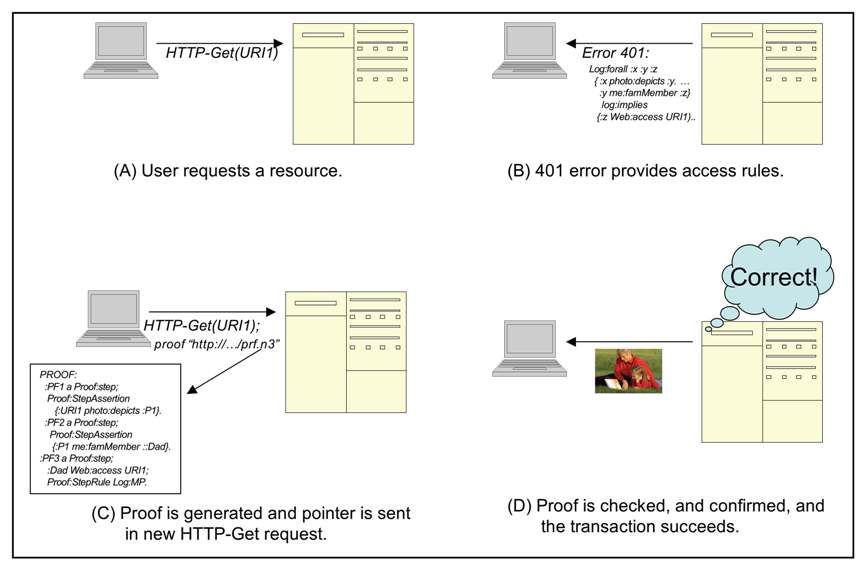
\epsfig{file=paw.jpg, height=5in}}

\caption{policy aware web scenario}\label{pawfig}

\end{figure}

\subsection{Automating Technical Reports}
  

\par CWM has also been used in the ``Technical Report Automation'' project.
This W3C project, based on the use of Semantic Web tools and
technologies, has allowed the streamlining the publication paper
trail of W3C Technical Reports, to maintain an RDF-formalized index
of these publications and to completely automate the maintenance of
the lists of Technical Reports.

\par The \empty W3C Technical Reports
index lists the formal work product of each W3C Working Group
categorized by one of six ``maturity levels''. The maturity
levels indicate the state of the work, from (first) working draft
to adopted standard (called ``W3C Recommendation''). The
\empty W3C Process
defines the formal steps necessary for a document to advance in
maturity level.

\par For many years the Technical Reports index had been maintained
manually and the critical workflow data that it contained was not
available in machine processable form. Checking the prerequisites
for each maturity advancement was entirely manual. Eventually, the
W3C pages listing the Working Groups, their chartered time periods,
their deliverables, and the Technical Reports index itself were all
turned into authoritative sources of Semantic Web data by adding
RDF markup to the existing HTML. The next step was to have data
extraction tools which in turn allowed cwm to check some of the
dependencies and prerequisites at the time a new document is
proposed for publication. The W3C Technical Reports index is now
built automatically by cwm and is available to users in multiple
views as well as in machine-processable RDF form, allowing a
variety of analyses to be performed.
\section{Related Work}
  

\par Euler is an inference engine supporting logic based proofs.
Unlike cwm, it is a backward-chaining reasoner enhanced with Euler
path detection.

\par Pychinko is a Python implementation of the classic Rete pattern
matching algorithm [REF]. Rete has shown to be, in many cases, the
most efficient way to apply rules to a set of facts--the basic
functionality of an expert system. Pychinko employs an optimized
implementation of the algorithm to handle facts, expressed as
triples, and process them using a set of N3 rules. Pychinko tries
to closely mimic the features available in Cwm, as it is one of the
most widely used rule engines in the RDF community. Pychinko has
proven to be faster than Cwm, however it's limitation lies in its
expressivity: Pychinko cannot handle most of the cwm builtins. It
is worth mentioning here that the RETE engine used in Pychinko has
been ported to Cwm - thus Cwm can now boast the same performance
improvements.
\section{Conclusion and Future Work}
  

\par The N3 language enabled our use of the Semantic Web both by its
simplicity and ease of use as a data language, and in the fact that
its extra expressive power allowed rules and rules about what
document said what to be written. The extra logical operations
added in Cwm to seemed to be a fairly complete set, in that new
applications were made by combining the old ones, and did not
require the constant additions of new builtins. That said, many
areas such as date and time processing, arithmetic for various
forms of number, and functions on lists and sets are covered quite
incompletely.

\par The cwm system is a useful, and much used, tool for many
practical small applications. However, it was not optimised for
speed, and as applications grow there are needs for cwm-compatible
fast processors for specific forms of problem. In general our
experience demonstrates both the need for and the adequacy of the
N3 formula as a quoting system for procesing of data in real
web-like environment, where the provenance of data is as important
a factor as its content.

\par Particularly interesting were applications in which a small N3
file caused cwm to find and integrate in real time data from
diverse sources on the web, and also small query files which cause
cwm to follow links to the point where the query can be resolved.
We hope in future to do more research into such systems which work
intimately and scalably in the Web.
\section{Acknowledgements}
  

\par This work was funded under @@@ DARPA and @@@ PAW NSF

\bibliography{index}


\end{document}
  